\chapter{Implementasi dan Pengujian}

Bab ini mecakup implementasi dan pengujian sistem hasil rancangan yang telah dijelaskan pada bab sebelumnya. Pada bab ini bagian implementasi tidak mencakup seluruh proses dan detail pada sistem. Detail tersebut dapat dilihat pada hasil implementasi (https://github.com/ibrohimislam/ngfilter). Sedangkan pada bab ini dijelaskan bagian menarik dari implementasi tersebut.

Pada bagian pengujian dijelaskan analisis pengujian yang memungkinkan dan alasan memilih pengujian. Pengujian yang dilakukan dengan transparent-firewall dipilih dengan alasan feasibilitas waktu yang dijelaskan pada bab ini. Kemudian dilanjutkan dengan hasil pengujian dan pembahasan.

\section{Arsitektur Implementasi Sistem}
Perancangan dilakukan dengan menggunakan framework NetFilter. NetFilter merupakan framework \textit{native} yang dimiliki oleh Linux untuk melakukan pemrosesan paket. Framework ini memberikan kemampuan untuk dapat menambahkan sebuah filter kepada user dengan berinteraksi dengan kakas pada \textit{userspace} yakni iptables.

\begin{figure}[H]
	\centering
	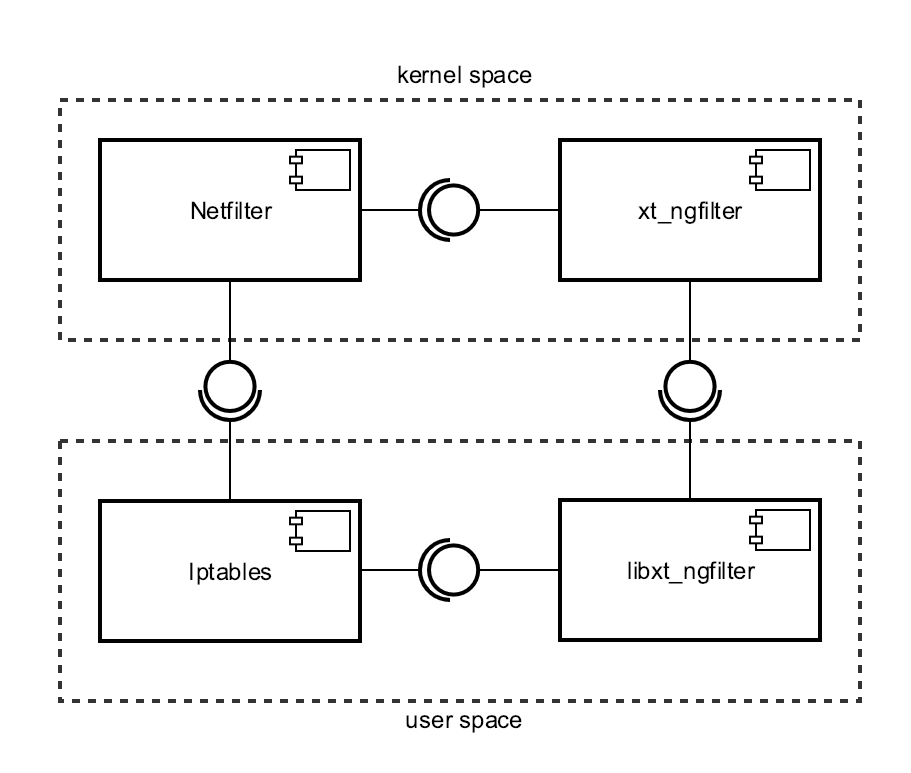
\includegraphics[width=230px]{resources/ngfilter_architecture.png}
	\caption{Arsitektur Pendekatan Dynamic}
	\label{fig:ngfilter_architecture}
\end{figure}

Secara garis besar arsitektur implementasi dapat dilihat pada diagram \ref{fig:ngfilter_architecture}. \verb|xt_ngfilter| dan \verb|libxt_ngfilter| merupakan bagian yang menjadi kontribusi implementasi dari tugas akhir ini. Dalam pemetaannya dengan arsitektur logicalnya, \verb|xt_ngfilter| merupakan implementasi komponen \textit{data interpreter} yang memiliki kemampuan DPI. Sedangkan \verb|libxt_ngfilter| merupakan implementasi komponen \textit{rule interpreter}.

Arsitektur implementasi sistem ini hanya memiliki 4 komponen, yakni: Netfilter, iptables,  \verb|xt_ngfilter|, dan \verb|libxt_ngfilter|. Komponen Netfilter pada sistem ini merupakan implementasi komponen \textit{data gatherer}, \textit{matcher}, \textit{filter}. Netfilter pada Linux memang diimplementasi untuk melakukan hal ini.

Bagian utama yang menjadi kontribusi adalah \verb|xt_ngfilter| dan \verb|libxt_ngfilter|. Bentuk diagram kelas nya dapat dilihat pada gambar \ref{fig:class_diagram}.

\begin{figure}[H]
	\centering
	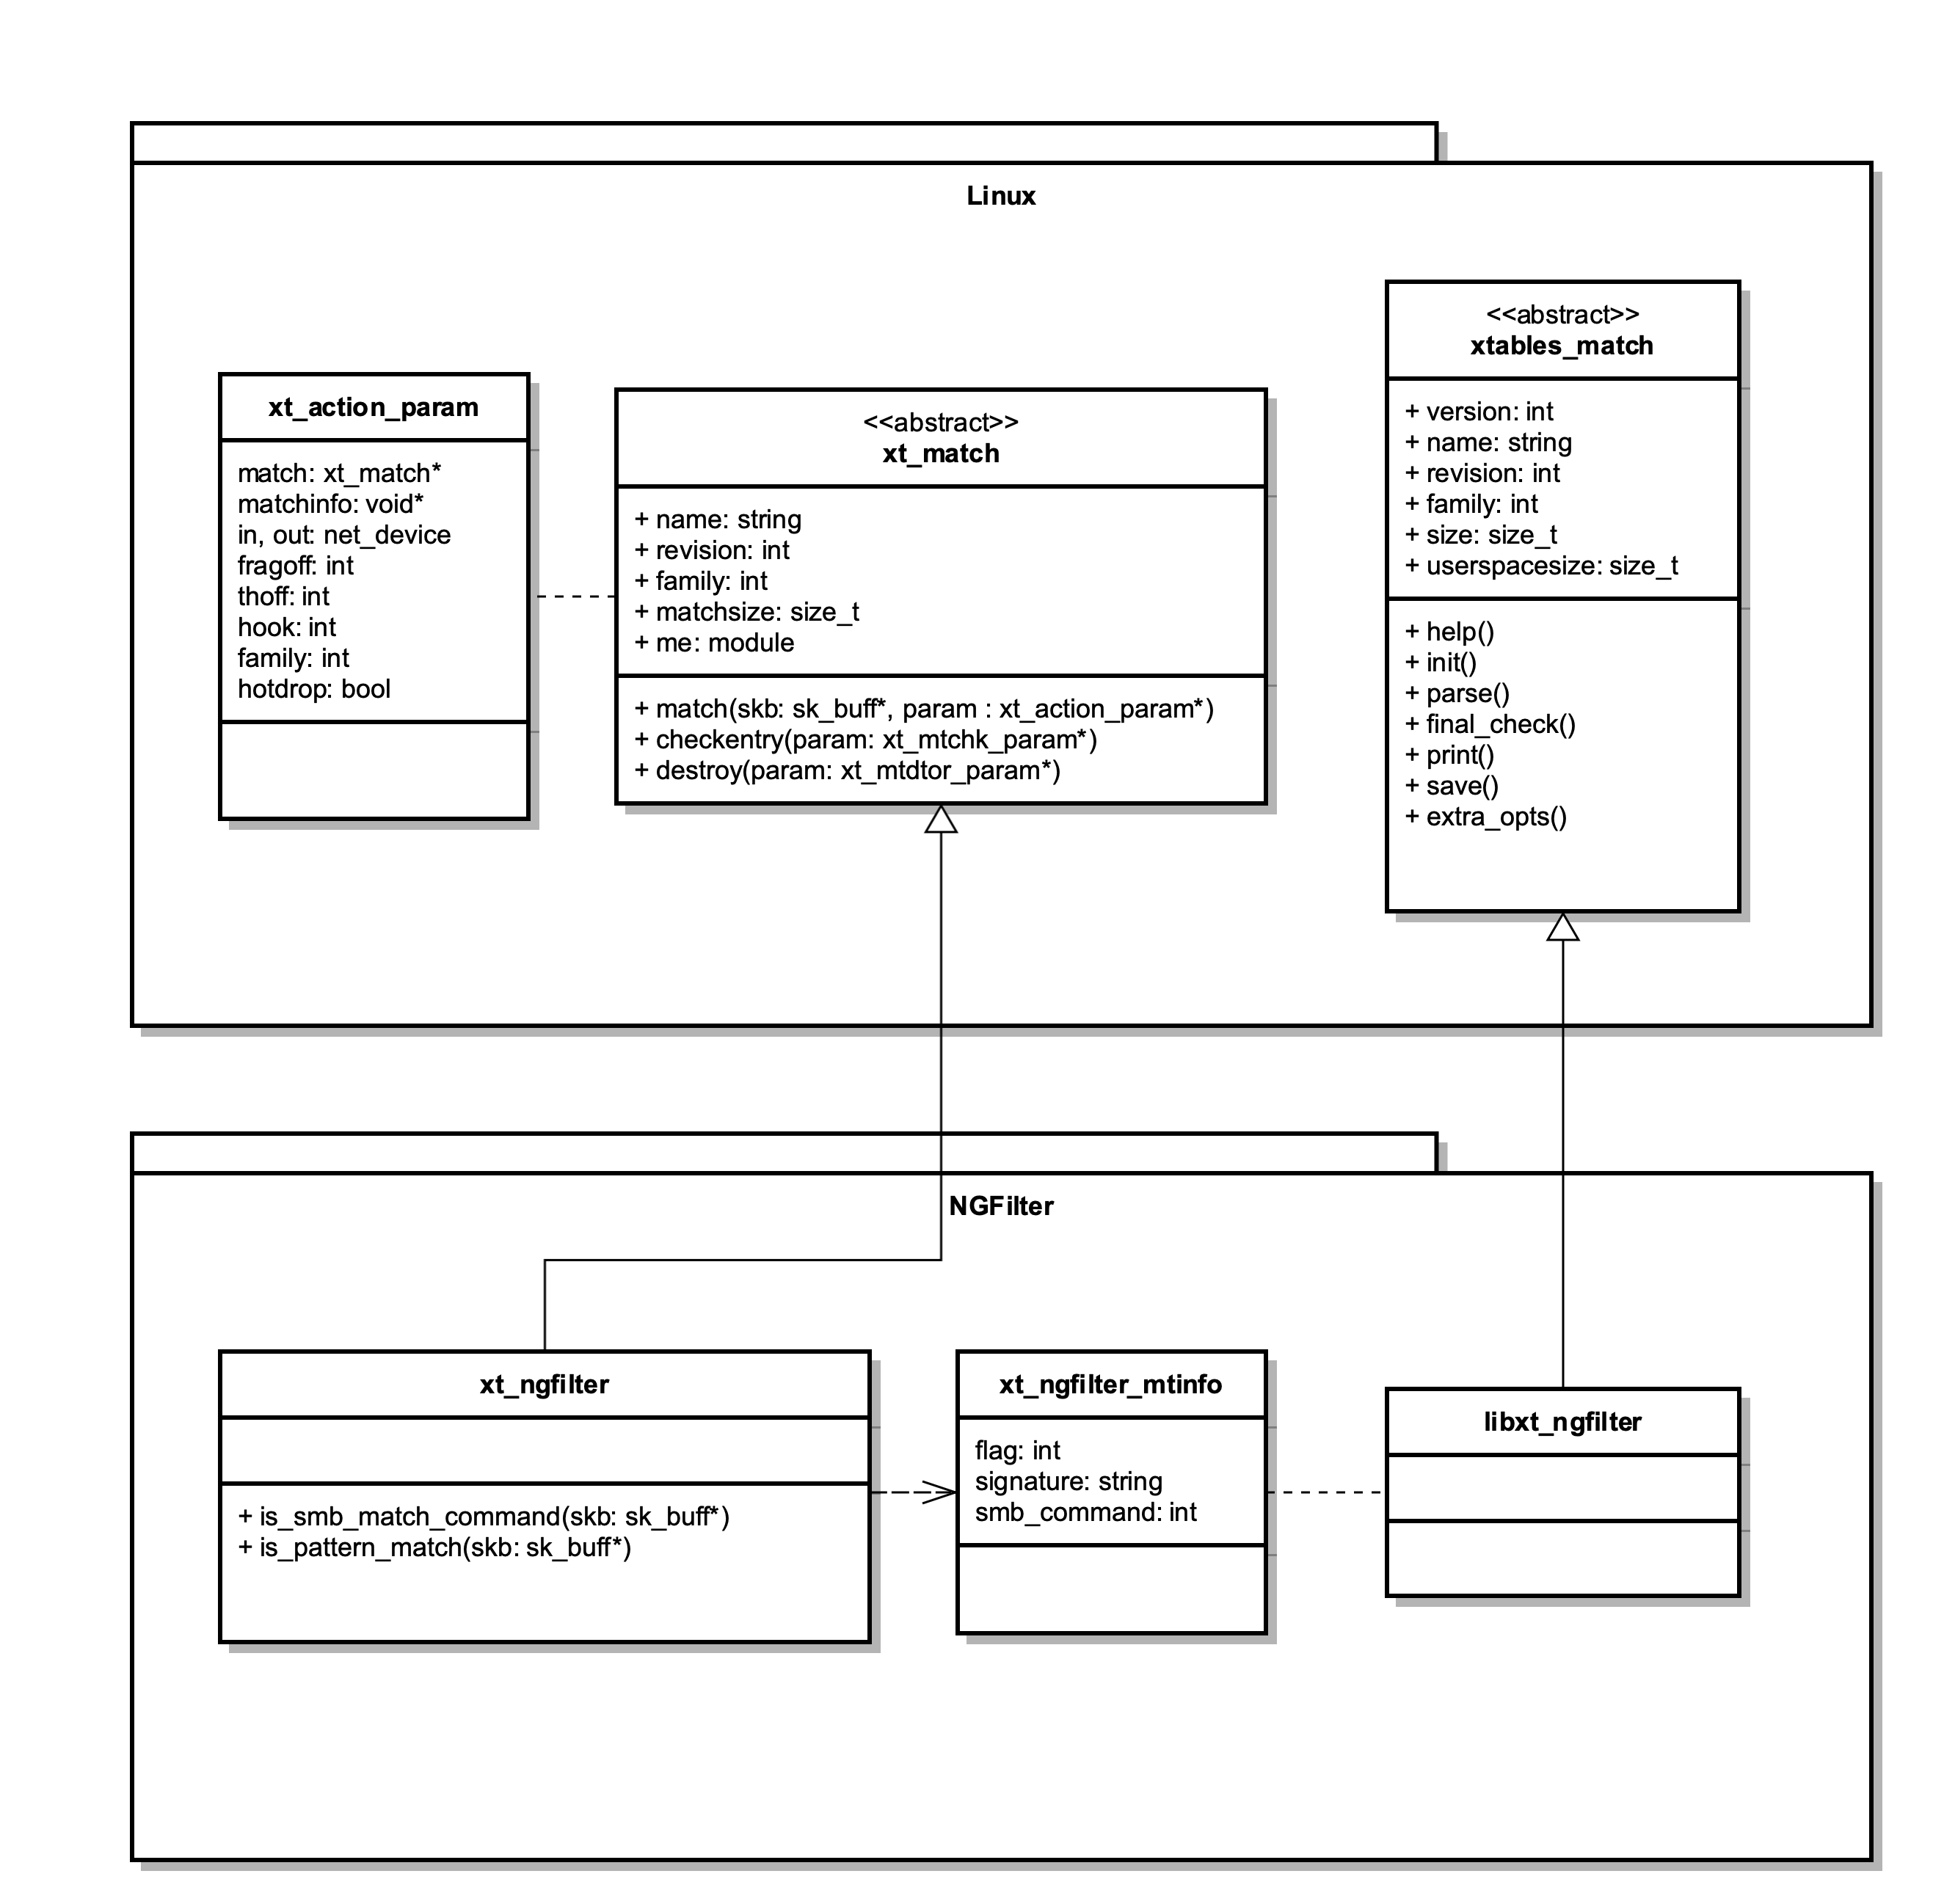
\includegraphics[width=370px]{resources/ngfilter_class_diagram.png}
	\caption{Diagram Kelas}
	\label{fig:class_diagram}
\end{figure}

\verb|xtables_match| merupakan sebuah struct yang memiliki properti \verb|help|, \verb|init|, \verb|parse|, \verb|final_check|, \verb|print|, \verb|save|, \verb|extra_opts| yang merupakan method yang akan diinvoke ketika melakukan manipulasi terhadap rule iptables.

\verb|xt_match| merupakan sebuah struct yang memiliki properti \verb|match|, \verb|checkentry|, dan \verb|destroy| yang akan diinvoke pada kernel space ketika sebuah paket melewati hook dan kemudian melakukan match terhadap modul yang diimplementasi. Fungsi \verb|match| merupakan bagian yang menentukan apakah sebauh packet match dengan parameter-parameter yang ada pada rule.


\section{Traceability Implementasi}

Pada tabel \ref{table:system_traceability_implementation} berikut ditunjukan kerunutan desain dan kebutuhan. Penangkalan paket (SR1) dapat menggunakan \textit{action} \verb|DROP| dari iptables. SR2, State machine dapat didipenuhi dengan menggunakan modul \verb|CONNTRACK| seperti dijelaskan pada subbab sebelumnya. SR3, deteksi protokol level aplikasi dapat dipenuhi dengan menggunakan modul nDPI-Netfilter. SR4, deteksi signature yang paham terhadap struktur data diimplementasi dalam bentuk modul kernel \verb|xt_ngfilter|. Kemudian untuk memenuhi SR5, menambahkan rule menggunakan kakas iptables dengan membuat modul \textit{userspace} untuk berinteraksi dengan modul kernel \verb|xt_ngfilter|.

\begin{table}[H]
	\caption{Traceability Implementasi Sistem}
	\label{table:system_traceability_implementation}
	\begin{tabularx}{\textwidth}{|l|X|X|}
		\hline
		\textbf{No} & \textbf{Kebutuhan} & \textbf{Desain} \\ \hline
		SR1 & Penangkalan paket & menggunakan action DROP oleh iptables\\ \hline 
		SR2 & State machine &  menggunakan modul mangle \verb|CONNTRACK| pada rule iptables \\ \hline
		SR3 & Deteksi protokol level aplikasi & menggunakan modul nDPI-NetFilter\\ \hline
		SR4 & Deteksi signature yang paham terhadap struktur data& class \verb|xt_ngfilter| pada diagram kelas \ref{fig:class_diagram} \\ \hline
		SR5 & Menambahkan rule & class \verb|libxt_ngfilter| pada diagram kelas \ref{fig:class_diagram} \\ \hline
	\end{tabularx}
\end{table}


\section{Implementasi ngfilter}

Implementasi dilakukan dengan membuat sebuah modul kernel \verb|xt_ngfilter| dan  \textit{shared library} \verb|libxt_ngfilter.so|.
Modul kernel digunakan untuk melakukan pencocokan, sedangkan \verb|libxt_ngfilter.so| berinteraksi dengan user melalui iptables.

\begin{lstlisting}
static struct xtables_match ngfilter_mt_reg = {
	.version = XTABLES_VERSION,
	.name = "ngfilter",
	.revision = 0,
	.family = NFPROTO_IPV4,
	.size = XT_ALIGN(sizeof(struct xt_ngfilter_mtinfo)),
	.userspacesize = XT_ALIGN(sizeof(struct xt_ngfilter_mtinfo)),
	.help = ngfilter_match_help,
	.init = ngfilter_match_init,
	.parse = ngfilter_match_parse,
	.final_check = ngfilter_match_check,
	.print = ngfilter_match_print,
	.save = ngfilter_match_save,
	.extra_opts = ngfilter_match_opts,
};
\end{lstlisting}

\begin{lstlisting}
static struct xt_match ngfilter_match4_reg __read_mostly = {
	.name = "ngfilter",
	.revision = 0,
	.family = NFPROTO_IPV4,
	.match = ngfilter_match,
	.checkentry = ngfilter_match_check,
	.destroy = ngfilter_match_destroy,
	.matchsize = sizeof(struct xt_ngfilter_mtinfo),
	.me = THIS_MODULE,
};
\end{lstlisting}

Instance struct \verb|xtables_match| digunakan untuk mendefinisikan modul match yang diimplementasi di userspace.
Property \verb|help|, \verb|init parse|, \verb|final_check|, \verb|print|, \verb|save|, dan \verb|extra_opts| merupakan \textit{function pointer} yang mengarah ke fungsi yang telah diimplementasi.

\begin{itemize}
\item \verb|ngfilter_match_init| dieksekusi saat modul di-\textit{register}.
\item \verb|ngfilter_match_exit| dieksekusi saat modul di-\textit{unregister}.
\item \verb|ngfilter_match_help| digunakan untuk menampilkan pesan bantuan ketika dipanggil dari \verb|iptables|.
\item \verb|ngfilter_match_parse| dieksekusi saat perintah dengan modul match \verb|ngfilter| ditambahkan ke rule. Fungsi ini melakukan mapping dari parameter perintah iptables ke dalam struktur data \verb|xt_ngfilter_mtinfo|.
\item \verb|ngfilter_match_check| merupakan fungsi yang dieksekusi saat melakukan validasi rule dengan menggunakan modul match \verb|ngfilter|.
\item \verb|ngfilter_match_print| merupakan fungsi untuk menampilkan rule yang sedang aktif. Fungsi ini dieksekusi ketika perintah \verb|iptables -L| dijalankan.
\item \verb|ngfilter_match_save| merupakan fungsi yang digunakan ketika perintah \verb|iptables-save| dijalankan. Fungsi ini melakukan mapping dari struktur data ke parameter perintah iptables sehingga dapat disimpan.
\end{itemize}

Berikut adalah definisi struct yang digunakan untuk berkomunikasi antara user-space dan kernel module.

\begin{lstlisting}
#define MAX_PATTERN_LENGTH 256
struct xt_ngfilter_mtinfo {
	unsigned char pattern[MAX_PATTERN_LENGTH];
	unsigned char smb_command;
	__u8 flags;
};
\end{lstlisting}

\section{Perancangan State Machine dengan Iptables}

Pada bagian ini dibahas bagaimana iptables dapat menjalankan state machine pada satu koneksi TCP. Hal ini digunakan pada perancangan selanjutnya untuk menjalankan \textit{rule} \textit{stateful} untuk mendapatkan \textit{signature} dari WannaCry. State machine dijalankan pada satu koneksi karena pada analisis ditemukan bahwa pada kasus WannaCry solusi ini cukup.

Kebutuhan yang diperlukan dalam melakukan implementasi state machine adalah sebagai berikut. state machine dapat menyimpan state; state machine dapat melakukan transisi state berdasarkan \textit{input} dan state saat ini; dan state machine dapat menentukan apakah sebuah \textit{input} dapat diterima atau tidak.

Implementasi penyimpanan state, dalam konteks ini state dalam satu koneksi TCP, dapat dilakukan denganmodul \verb|CONNTRACK| pada iptables yang dapat menyimpan state dalam bentuk 32-bit. Modul \verb|CONNTRACK| dapat digunakan pada tabel \verb|MANGLE|. Berikut adalah perintah yang dapat digunakan.

\begin{lstlisting}
-t mangle -A PREROUTING -j CONNMARK --restore-mark
-t mangle -A POSTROUTING -j CONNMARK --save-mark
\end{lstlisting} 

Perintah di atas dapat menyimpan tanda yang diatur dengan modul \verb|MARK|, dan mengembalikannya tanda pada paket selanjutnya. Akibatnya seluruh tanda yang ada pada sebuah paket akan menjadi state koneksi ketika masuk ke chain \verb|POSTROUTING|. Kemudian seluruh paket yang masuk setelah koneksi memiliki state, akan ditandai ketika masuk ke chain \verb|PREROUTING|.

Implementasi transisi state dapat dilakukan dengan modul \verb|MARK|. Hal ini dapat dilakukan dengan cara melakukan pengecekan terhadap tanda pada paket dan mengubah tanda jika menemukan kondisi yang cocok. Berikut adalah perintah yang dapat digunakan untuk melakukan transisi state.

\begin{lstlisting}
-m mark --mark $CURRENT_STATE $ALPHABET -j MARK --set-xmark $NEW_STATE
\end{lstlisting}

Perintah di atas akan melakukan pengecekan bahwa sebuah paket berada dalam sebuah state \verb|$CURRENT_STATE| dan menerima \textit{input} berupa \verb|$ALPHABET|. Kemudian ketika kondisi tersebut dipenuhi, maka tanda akan diubah ke \verb|$NEW_STATE|. Sehingga perintah tersebut dapat merepresentasikan fungsi transisi state.

Implementasi state machine dapat menerima sebuah \textit{input} atau tidak dapat dilakukan dengan menggunakan perintah \verb|-j $ACTION|. Perintah itu harus dipasangkan setelah melakukan pengecekan terhadap state final. Bentuk lengkap perintahnya adalah sebagai berikut.

\begin{lstlisting}
-m mark --mark $FINAL_STATE -j $ACTION
\end{lstlisting}

\section{Implementasi Rule iptables}

Penangkalan paket \textit{malicious} dapat dilakukan dengan menggunakan rule iptables dengan menambahkan modul yang telah diimplementasi sesuai desain pada subbab III.6. Penangkalan paket \textit{malicious} dapat ditangani dengan menggunakan modul \verb|ndpi-netfilter| dan modul \verb|ngfilter| dengan rule iptables sebagai berikut:

\begin{lstlisting}
-t mangle -A PREROUTING -j CONNMARK --restore-mark
-t mangle -A POSTROUTING -j CONNMARK --save-mark
-A FORWARD -m ndpi --smb  -m ngfilter --smb-command a0 -j MARK --set-xmark 0x1/0xffffffff
-A FORWARD -m mark --mark 0x1 -j LOG --log-prefix "MARK 1: "
-A FORWARD -m mark --mark 0x1 -m ngfilter --smb-command 33 -j MARK --set-xmark 0x2/0xffffffff
-A FORWARD -m mark --mark 0x2 -j LOG --log-prefix "MARK 2: "
-A FORWARD -m mark --mark 0x2 -j DROP
\end{lstlisting} 

\section{Analisis Pengujian}

Berkaitan dengan cara penyebaran worm, terdapat 2 penempatan firewall yang perlu diperhatikan, yaitu firewall di antara subnet dan firewall dalam sebuah subnet. Penempatan ini berbeda perilakunya jika dilihat dari sifat worm yang melakukan \textit{local-scanning} dan \textit{random-scanning}. Kedua jenis penempatan dapat mendeteksi random-scanning namun tidak dapat mendeteksi \textit{local-scanning}.

Firewall di antara subnet merupakan firewall yang bekerja sebagai router (layer TCP/IP) sekaligus melakukan filtering. Firewall umumnya ditemukan dengan penempatan ini. Firewall dengan penempatan ini dapat melakukan penjagaan lalu lintas antar subnet. Namun tidak dapat menjamin pengamanan antar host dalam subnet tersebut. Sehingga, jika terdapat host yang terinfeksi worm dan melakukan \textit{subnet-local-scanning} firewall tidak dapat mendeteksi aktivitas tersebut.

Cara penempatan firewall pada sebuah subnet dapat melakukan penjagaan pada sekelompok host dan memisahkannya dari host yang lain dalam sebuah subnet. Firewall dengan penempatan ini umumnya disebut \textit{transparent firewall}. Penempatan ini dapat mendeteksi aktivitas \textit{subnet-local-scanning} jika melintasi firewall.

Karena dibatasi waktu, pengujian dengan menempatkan firewall di antara subnet tidak dapat dilakukan karena memerlukan sumber daya dan waktu yang tidak dapat dipenuhi.  Keadaan tersebut dapat diperkirakan seperti persamaan \ref{eqn:prob_one}-\ref{eqn:expected_time}.

Jika seperti pada persamaan \ref{eqn:prob_one}, $P(1)$ adalah kemungkinan kemunculan sebuah ip maka $P(n)$ (persamaan \ref{eqn:prob_n}) merupakan kemungkinan muncul salah satu dari n ip. Sehingga diperlukan ekspektasi percobaan yang diperlukan untuk menemukan ip adalah $E(n)$ kali percobaan (persamaan \ref{eqn:expectation_n}). Jika kecepatan \textit{scanning} adalah $v(1)$ dan kecepatan m buah host adalah $v(m)$, $v(m)$ dapat didekati dengan m kali $v(1)$ (persamaan \ref{eqn:velocity_m}). Jika perkiraan waktu yang dibutuhkan untuk menemukan 1 dari n ip, dengan m host yang melakukan percobaan dengan kecepatan $v(1)$ adalah $t(n,m)$, maka waktu yang dibutuhkan adalah jumlah percobaan yang diperlukan dibagi dengan kecepatan.

Dari pengamatan yang dilakukan kecepatan \textit{scanning} secara acak adalah 1064 ip per menit. Maka dengan persamaan \ref{eqn:expected_time} dengan 32 host terinfeksi dan 32 host target dibutuhkan 3 hari untuk mendapatkan satu serangan. Jika 1 serangan dianggap satu data maka untuk mendapatkan 10 data setidaknya diperlukan waktu 30 hari.

\begin{equation}
\label{eqn:prob_one}
P(1) = \frac{1}{2^{32}-1}
\end{equation}

\begin{equation}
\label{eqn:prob_n}
P(n) = \frac {n}{2^{32}-1}
\end{equation}

\begin{equation}
\label{eqn:expectation_n}
E(n) = \frac{1}{P(n)} = \frac{2^{32}-1}{n}
\end{equation}

\begin{equation}
\label{eqn:velocity_m}
v(m) \approx m \times v(1)
\end{equation}

\begin{equation}
\label{eqn:expected_time}
t(n,m) = \frac{E(n)}{v(m)} \approx \frac{2^{32}-1}{n \times m \times v}
\end{equation}

\section{Skenario Pengujian Akurasi}

Pengujian dilakukan menggunakan membandingkan hasil percobaan kontrol dengan percobaan yang menggunakan firewall hasil implementasi. Percobaan dilakukan pada sebuah \textit{hypervisor} yang memiliki spesifikasi pada tabel \ref{table:hypervisor_specification}. Percobaan ini dilakukan dengan menggunakan 10 virtual machine yang tidak terinfeksi, 1 virtual machine yang telah terinfeksi dan 1 firewall.

\begin{table}[H]
	\caption{Spesifikasi hypervisor yang digunakan untuk melakukan pengujian}
	\label{table:hypervisor_specification}
	\begin{tabularx}{\textwidth}{|l|X|}
		\hline
		\textbf{Spesifikasi} & \textbf{Spesifikasi yang digunakan} \\ \hline
		\textit{Processor} & Intel(R) Xeon(R) CPU E5-2620 0 @ 2.00GHz \\ \hline 
		\textit{Virtualization Infrastructure} & Qemu/KVM \\ \hline
		Linux & Linux 3.10.0-862.11.6.el7.x86\_64 \#1 SMP Tue Aug 14 21:49:04 UTC 2018 x86\_64 x86\_64 x86\_64 GNU/Linux \\ \hline
	\end{tabularx}
\end{table}


Percobaan dilakukan dengan memisahkan sebuah subnet 192.168.1.0/24 menjadi dua bagian,\textit{internal\_network} dan \textit{external\_network} seperti pada gambar \ref{fig:validation_scenario}. Kedua bagian tersebut kemudian dihubungkan dengan sebuah transparent firewall. Kemudian masing-masing bagian ditempatkan 5 host. \textit{external\_network} ditempatkan 5 host untuk menunjukkan bahwa WannaCry dapat menginfeksi host-host yang berada pada jaringan yang sama. 

Percobaan kontrol dan percobaan firewall hasil implementasi akan memperlakukan \textit{internal\_network} dengan berbeda. Jika pada percobaan kontrol, firewall tidak menerapkan \textit{rule} sama sekali pada chain FORWARD. Sedangkan pada percobaan firewall hasil implementasi akan menerapkan \textit{rule} hasil implementasi. Sehingga hasil percobaan dapat menunjukkan bagaimana perilaku malware akibat \textit{rule} yang diterapkan.

Untuk mendapatkan data perilaku host-host baik pada \textit{internal\_network} maupun \textit{external\_network} pada firewall dilakukan \textit{packet capture}. Packet capture tersebut diharapkan dapat menjelaskan keadaan network eksternal dan network internal. Keadaan penting yang perlu dilakukan pengamatan adalah kapan sebuah host terinfeksi. Dengan menggunakan definisi host terinfeksi yang telah dijelaskan sebelumnya, seharusnya dapat dideteksi ketika sebuah host mulai melakukan \textit{local-scanning}.

Seluruh proses pengambilan data menggunakan script otomasi yang dijelaskan pada lampiran A. Masing-masing percobaan dilakukan 30 menit dengan menempatkan sebuah host terinfeksi pada \textit{external\_network} pada detik ke 30. Kemudian setelah 30 menit \textit{packet capture} dihentikan dan seluruh host diatur ulang dengan melakukan \textit{cloning} host yang telah disediakan.

\begin{figure}[H]
	\centering
	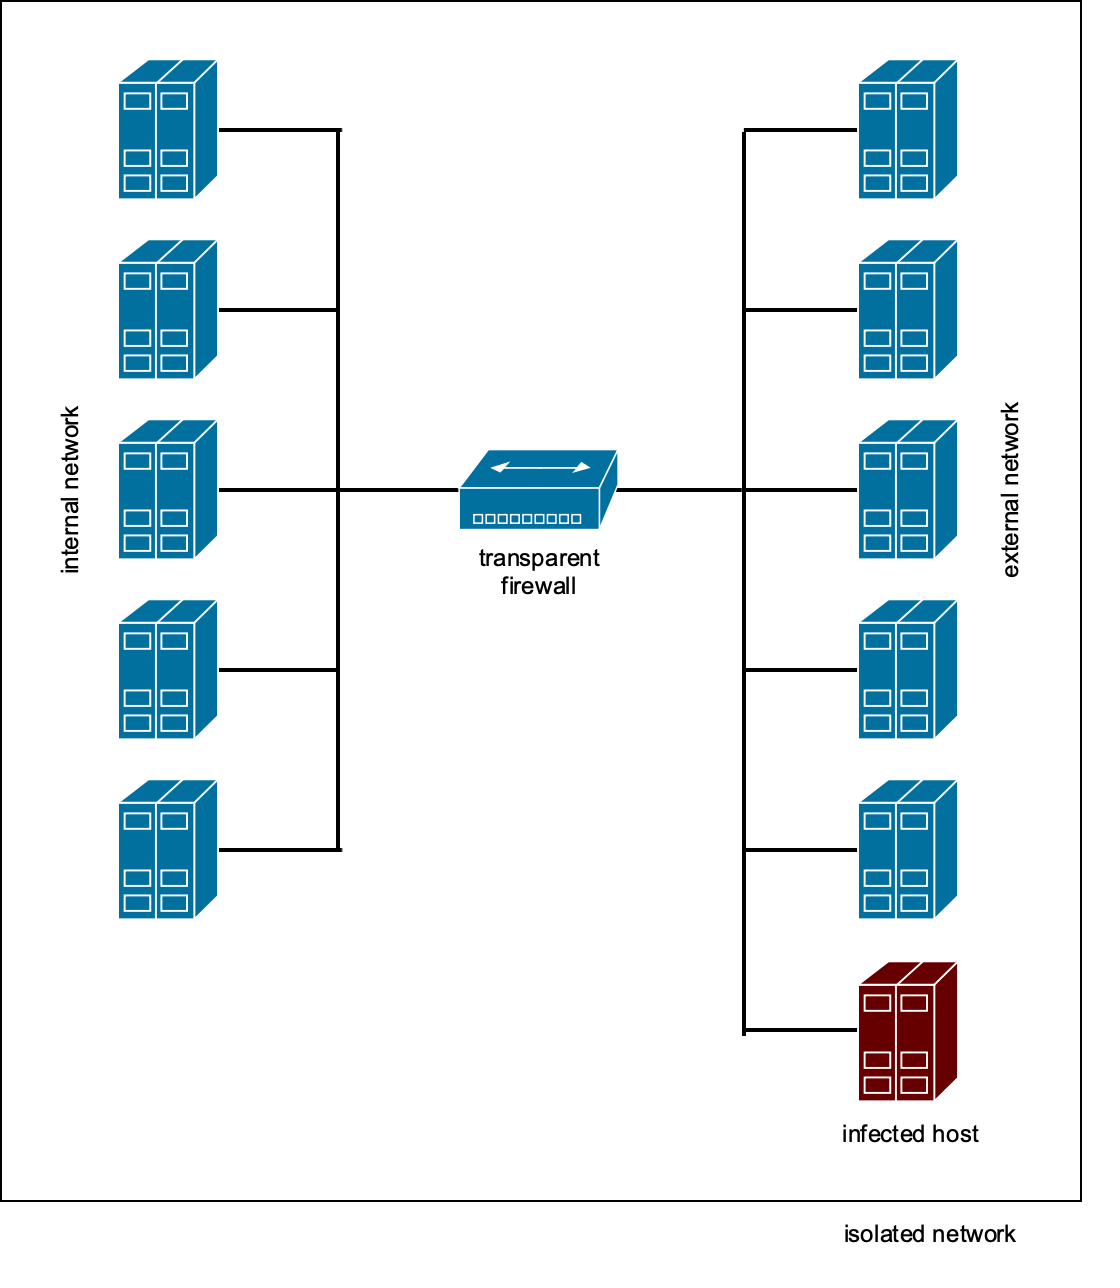
\includegraphics[width=180px]{resources/skenario_pengujian.png}
	\caption{Susunan jaringan skenario pengujian}
	\label{fig:validation_scenario}
\end{figure}

\section{Hasil Pengujian Akurasi}

Data dari hasil percobaan berbentuk file pcap (\textit{packet capture}) dilakukan pengolahan untuk mendapatkan perkiraan waktu host terinfeksi. Hasil pengolahan data dapat dilihat di Lampiran B berisi data perkiraan waktu host terinfeksi. Kemudian data tersebut diakumulasikan untuk setiap percobaan untuk mendapatkan data pada suatu waktu telah ada berapa host terinfeksi.

\begin{figure}[H]
	\centering
	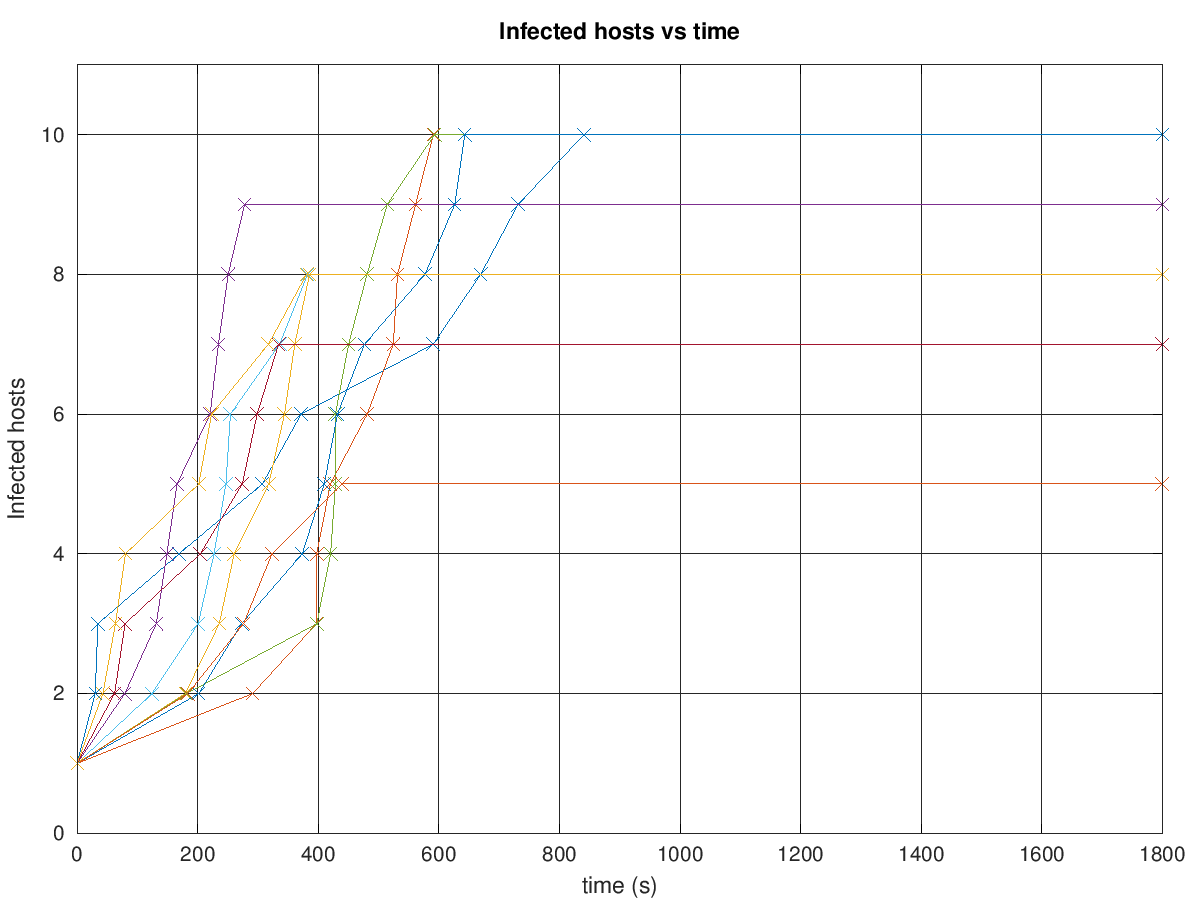
\includegraphics[width=\textwidth]{resources/infection_control_over_time.png}
	\caption{Grafik host terinfeksi terhadap waktu (percobaan kontrol)}
	\label{fig:infection_control_over_time}
\end{figure}

Grafik akumulasi host terinfeksi pada percobaan kontrol dapat dilihat pada gambar \ref{fig:infection_control_over_time}. Grafik tersebut berisi 10 data percobaan kontrol. Dari 10 percobaan tersebut dapat diperkirakan setelah 900 detik sudah terdapat lebih dari 5 host terinfeksi baik dari \textit{internal\_network} maupun \textit{external\_network}.

\begin{table}[H]
	\caption{Akumulasi detik ke-1800 host terinfeksi (percobaan kontrol)}
	\label{table:1800s_all_network_control}
	\begin{center}
		\begin{tabularx}{300px}{|X|r|}
			\hline
			\multicolumn{1}{|l}{\textbf{Jumlah host terinfeksi}} & \multicolumn{1}{|l|}{\textbf{Teramati}} \\ \hline
			5 & 1 percobaan\\ \hline
			7 & 1 percobaan\\ \hline
			8 & 3 percobaan\\ \hline
			9 & 1 percobaan\\ \hline
			10 & 4 percobaan\\ \hline
		\end{tabularx}
	\end{center}
\end{table}

\begin{table}[H]
	\caption{Akumulasi detik ke-1800 host \textit{internal\_network} terinfeksi (percobaan kontrol)}
	\label{table:1800s_internal_network_control}
	\begin{center}
		\begin{tabularx}{300px}{|X|r|}
			\hline
			\multicolumn{1}{|l}{\textbf{Jumlah host \textit{internal\_network} terinfeksi}} & \multicolumn{1}{|l|}{\textbf{Teramati}} \\ \hline
			2 & 1 percobaan\\ \hline
			3 & 1 percobaan\\ \hline
			4 & 4 percobaan\\ \hline
			5 & 4 percobaan\\ \hline
		\end{tabularx}
	\end{center}
\end{table}

Pada tabel \ref{table:1800s_all_network_control} dapat dilihat persebaran hasil pengamatan host terinfeksi pada \textit{internal\_network} maupun \textit{external\_network}. Sedangkan pada tabel \ref{table:1800s_internal_network_control} dapat dilihat persebaran pengamatan host terinfeksi pada \textit{internal\_network}. Kedua distribusi ini dapat menggambarkan perilaku infeksi WannaCry.

\begin{table}[H]
	\caption{Akumulasi detik ke-1800 host terinfeksi (percobaan firewall implementasi)}
	\label{table:1800s_all_network_firewalled}
	\begin{center}
		\begin{tabularx}{300px}{|X|r|}
			\hline
			\multicolumn{1}{|l}{\textbf{Jumlah host terinfeksi}} & \multicolumn{1}{|l|}{\textbf{Teramati}} \\ \hline
			1 & 40 percobaan\\ \hline
			2 & 15 percobaan\\ \hline
			3 & 16 percobaan\\ \hline
			4 & 3 percobaan\\ \hline
			5 & 8 percobaan\\ \hline
			4 & 1 percobaan\\ \hline
		\end{tabularx}
	\end{center}
\end{table}

\begin{figure}[H]
	\centering
	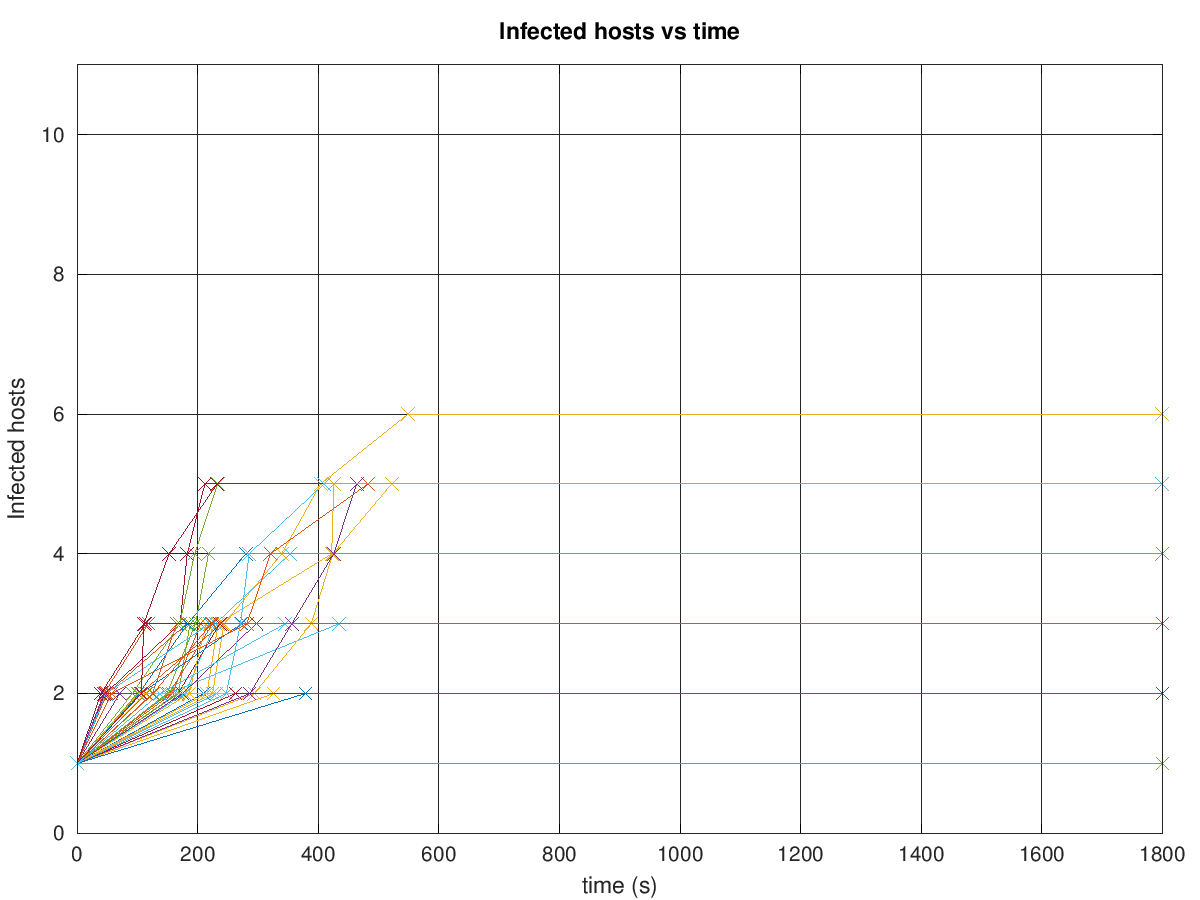
\includegraphics[width=\textwidth]{resources/infection_control_over_time_firewalled.png}
	\caption{Grafik host terinfeksi terhadap waktu (percobaan implementasi firewall)}
	\label{fig:infection_control_over_time_firewalled}
\end{figure}

Grafik akumulasi host terinfeksi pada percobaan implementasi firewall dapat dilihat pada gambar \ref{fig:infection_control_over_time_firewalled}. Pada gambar tersebut diamati setelah detik ke-600 tidak terjadi infeksi. Jumlah maksimum infeksi yang terjadi sebanyak 6 host yakni host pada \textit{external\_network}. Persebaran pengamatan host terinfeksi pada keseluruhan network dapat dilihat pada tabel \ref{table:1800s_all_network_firewalled}. Dari 83 percobaan tidak diamati infeksi terjadi pada \textit{internal\_network}.

\section{Skenario Pengukuran Kinerja}

Pengujian performa dilakukan dengan menggunakan kakas \verb|iperf3| dengan versi \verb|3.1.3-1|. Pengujian dapat kinerja dapat dilakukan pada sembarang protokol TCP karena kinerja iptables tidak akan dipengaruhi oleh protokol. Kinerja iptables bergantung pada banyaknya \textit{rule} dan seberapa kompleks algoritma match dari masing-masing modul yang digunakan.

Seperti yang dilakukan sebelumnya, pengukuran dilakukan dengan dua percobaan yakni percobaan kontrol dan percobaan firewall hasil implementasi. Pengujian ini bertujuan untuk menunjukkan seberapa besar penurunan kinerja sistem akibat \textit{rule} yang diterapkan. Sehingga pada percobaan kontrol \textit{rule} tidak diterapkan sedangkan pada percobaan firewall hasil implementasi \textit{rule} diterapkan. Masing-masing percobaan dilakukan selama 100 detik. 

Terdapat dua host yakni 192.168.1.111 dan 192.168.1.112. 192.168.1.111 berada pada \textit{internal\_network} dan 192.168.1.112 berada pada \textit{external\_network} Perintah berikut dijalankan pada host 192.168.1.111:
\begin{lstlisting}
iperf3 -s
\end{lstlisting}

\noindent Kemudian perintah berikut dijalankan pada host 192.168.1.112:
\begin{lstlisting}
iperf3 -c 192.168.1.111 -p 5201 -t 100 --logfile output.txt
\end{lstlisting}


\section{Hasil Pengukuran Kinerja}

Dua percobaan tersebut menghasilkan data bandwidth dan data \textit{packet retry}. Hasil pengukuran \textit{bandwidth} dapat dilihat pada gambar \ref{fig:bandwidth_boxplot}. Hasil pengukuran \textit{packet retry} dapat dilihat pada gambar \ref{fig:retr_boxplot}.

\begin{figure}[H]
	\centering
	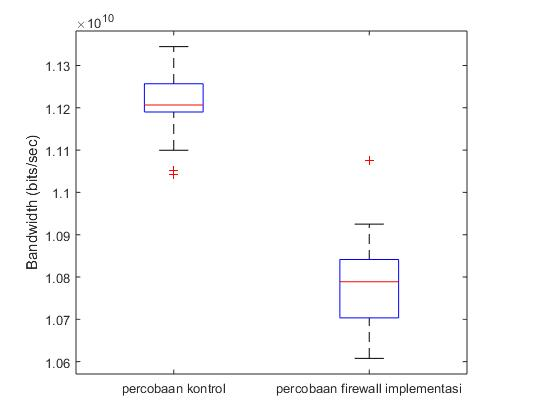
\includegraphics[width=250px]{resources/bandwidth_boxplot.jpg}
	\caption{Perbandingan bandwidth}
	\label{fig:bandwidth_boxplot}
\end{figure}

\begin{figure}[H]
	\centering
	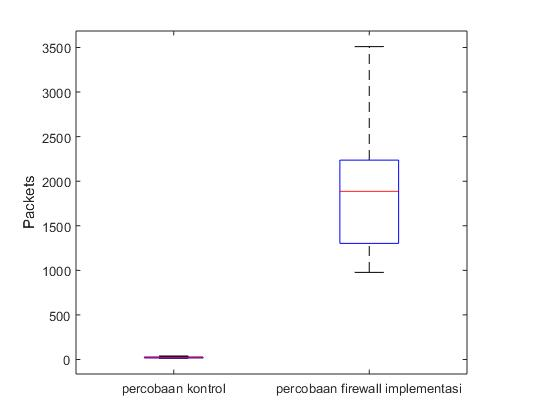
\includegraphics[width=250px]{resources/retr_boxplot.jpg}
	\caption{Perbandingan packet retry}
	\label{fig:retr_boxplot}
\end{figure}

Pada data \textit{bandwidth} 30 data hasil pengukuran untuk masing-masing percobaan, menunjukkan penurunan rata-rata bandwidth sebesar 4\%. Sedangkan pada rata-rata \textit{packet retry} diamati kenaikan lebih besar dari 8202\%. Hal ini menunjukkan memang ada penurunan kinerja akibat diterapkannya firewall ini.

\section{Pembahasan}

Pada subbab ini dijelaskan bagaimana tujuan pada bab I berhasil dilakukan berdasarkan data yang didapatkan pada percobaan. Selain itu dalam subbab ini dijelaskan kelemahan dan kemungkinan pengembangan selanjutnya. Kelemahan dan kemungkinan pengembangan selanjutnya yang kemudian disimpulkan dalam bab selanjutnya.

Percobaan kontrol menunjukkan bahwa malware WannaCry tetap dapat menginfeksi meskipun melalui sebuah \textit{bridge}, dalam hal ini juga berlaku sebagai \textit{transparent firewall} namun belum diterapkan \textit{rule}. Percobaan ini menunjukkan pada kondisi tanpa perlakuan, WannaCry dapat menginfeksi \textit{internal\_network}. Jika implementasi dapat mencapai mencegah penyebaran WannaCry maka dengan perlakuan tersebut seharusnya WannaCry tidak dapat menginfeksi \textit{internal\_network}.

Kemudian hasil percobaan firewall implementasi dari 83 data yang diamati, tidak terjadi infeksi pada \textit{internal\_network}. Data tersebut membuktikan bahwa implementasi firewall dapat mencegah infeksi WannaCry dengan signifikan. Meskipun dari 83 data masih belum diamati \textit{false-negative}. \textit{False-negative} seharusnya dapat diamati ketika terjadi infeksi pada \textit{internal\_network}.

Selain itu \textit{false-positive} juga sulit diamati dari data tersebut karena pengujian hanya memperhatikan bagaimana infeksi terjadi. Sedangkan tidak melakukan pengecekan pada protokol SMB pada keadaan normal. Walaupun penulis telah melakukan pengujian pada saat implementasi, dan mengamati bahwa rule firewall tersebut tidak mengganggu proses normal.

Bagian menarik dari data pada Lampiran B, malware ini tidak menginfeksi \textit{external\_network} secara maksimal ketika rule diterapkan. Dari hal ini dapat ditarik sebuah kesimpulan ketika malware ditangani pada suatu sisi, sisi lain dari \textit{network} pun menjadi lebih aman. Hal ini terjadi karena \textit{internal\_network} tidak menjadi host yang terinfeksi dan kemudian ikut menyerang host lain.

Implementasi dalam bentuk \textit{signature-based} memiliki kelebihan untuk dapat menangkap signature dengan tingkat \textit{false-negative} yang kecil. Implementasi pada iptables merupakan bentuk implementasi \textit{realtime dynamic signature-based detection}. Implementasi DPI dalam bentuk ini perlu memperhatikan fragmentasi paket, sehingga paket perlu ditunggu hingga lengkap untuk dapat dianalisis. Pada implementasi saat ini masih belum secara detail diperhatikan, sehingga memungkinkan untuk menimbulkan \textit{false-negative}.

Pemilihan \textit{signature} dengan menggunakan \textit{vulnerability} yang di-\textit{exploit} malware dapat menimbulkan \textit{false-positive}. \textit{False-positive} ini terjadi ketika serangan dari malware lain atau attacker yang menggunakan vulnerability yang digunakan pada deteksi. Sehingga hal ini tidak dapat mendeteksi secara presisi serangan yang dideteksi merupakan serangan oleh WannaCry.

Pada pengembangan selanjutnya, seharusnya implementasi dalam bentuk ini dapat digunakan untuk mendeteksi signature malware-malware yang telah diketahui. Hal ini seharusnya dapat menekan \textit{long-tail infection} yang terjadi seperti pada malware WannaCry ini. Namun, tidak semua malware dapat dideteksi dengan implementasi ini. Hal ini karena tidak semua signature infeksi dapat ditemukan dalam satu koneksi seperti yang terjadi pada WannaCry. Oleh karena itu diperlukan implementasi state-machine yang tidak hanya \textit{single-connection oriented}.

Hasil pengukuran kinerja menujukan perbedaan yang dapat diterima dan penurunan tidak signifikan pada bandwidth. Sedangkan pada \textit{packet retry}, terlihat perbedaan yang signifikan antara percobaan kontrol dan percobaan firewall implementasi. Hal ini terjadi karena firewall implementasi memang memerlukan pemrosesan tambahan ketika menerima paket. Penurunan performa ini dalam kadar yang dapat diterima.

\section{Permasalahan Teknis}

Dalam subbab ini dijelaskan hal-hal apa saja yang menjadi beberapa hambatan dalam melakukan implementasi DPI pada firewall. Beberapa masalah mengenai dokumentasi dan permasalahan library yang digunakan, hingga pada proses pengujian.

Hambatan paling dirasakan adalah kurangnya dokumentasi mengenai perubahan yang harus dilakukan untuk modul kernel untuk berubah ke versi yang lebih tinggi. Salah satu akibatnya adalah meski pun tersedia panduan pembuatan modul kernel untuk Netfilter namun karena perbedaan versi tidak dapat dilakukan dengan mudah.

Selain itu implementasi nDPI saat ini merupakan implementasi pada userspace sehingga tidak dapat dengan mudah digunakan pada modul kernel. Pada versi terdahulu nya nDPI memang dapat digunakan pada kernel. Namun pada versi terbaru, sudah tidak men-\textit{support} penggunakan pada kernel. Sehingga diperlukan beberapa patch untuk mengubah library-library userspace yang digunakan nDPI.

Pengujian dengan menggunakan transparent firewall di satu sisi dapat mempermudah dalam mendapatkan data. Namun, pada sisi teknisnya karena transparent firewall dalam implementasinya berupa bridge yang beroperasi pada layer 2. Sedangkan iptables beroperasi pada layer 3. Diperlukan pengaturan khusus pada kernel sehingga forwarding pada layer 2 dapat mengaktifkan hook pada iptables.